\documentclass{ucll-slides}
\usepackage{pxfonts}
\usepackage{tikz}
\usepackage{calc}
\usepackage{ucll-code}


\usetikzlibrary{calc,shadows,tikzmark}
\beamertemplatenavigationsymbolsempty

\coursename{Distributed Applications}
\title{Processes}

\pgfkeys{
  /envelope/.cd,
  width/.initial=1cm,
  height/.initial=0.8cm,
  position/.initial={0,0},
  value/.initial={},
  value font/.initial={\ttfamily}
}

\tikzset{
    note/.style={drop shadow,fill=green!50,inner sep=5mm},
    note2/.style={drop shadow,fill=cyan!50,inner sep=5mm},
    note arrow/.style={-latex,ultra thick}
}

\newcommand{\envelope}[1][1]{
    {
        \pgfkeys{/envelope/.cd,#1}
        \pgfkeys{/envelope/width/.get=\envwidth}
        \pgfkeys{/envelope/height/.get=\envheight}
        \pgfkeys{/envelope/position/.get=\envposition}
        \draw[fill=white] (\envposition) rectangle ++(\envwidth,\envheight);
        \draw[fill=white] (\envposition) -- ++(\envwidth * 0.5,\envheight * 0.6) -- ++(\envwidth * 0.5,-\envheight * 0.6) -- cycle;
        \draw[fill=white] ($ (\envposition) + (0,\envheight) $) -- ++(\envwidth * 0.5,-\envheight * 0.6) -- ++(\envwidth * 0.5,\envheight * 0.6) -- cycle;
    }
}

\newcommand{\csharp}{C$^\sharp$}

\newcommand{\codeunderlinex}[2][]{
  \codeunderline[name center=#2,#1]{#21}{#22}
}

\newcommand{\codeoverlinex}[2][]{
  \codeoverline[name center=#2,#1]{#21}{#22}
}

\begin{document}

\maketitle

\section{OS Refresher}

\frame{\tableofcontents[currentsection]}

\begin{frame}
    \frametitle{Operating Systems Refresher}
    \begin{center}
        \begin{tikzpicture}[scale=0.8,transform shape,
                            os/.style={draw,drop shadow,fill=blue!50},
                            process/.style={draw,drop shadow,fill=red!50},
                            process header/.style={font=\sc\bf\Large,red,opacity=0.5},
                            hardware/.style={drop shadow,fill=magenta!50},
                            cpu/.style={draw,minimum width=1cm,minimum height=1cm,drop shadow,fill=magenta!75}]
            \node[os,minimum width=10cm,minimum height=1cm] (os) {Operating System};
            \coordinate (process a) at ($ (os.south west) + (0,-0.2) $);
            \coordinate (process b) at ($ (os.south west) ! 0.35 ! (os.south east) + (0,-0.2) $);
            \coordinate (process c) at ($ (os.south west) ! 0.7 ! (os.south east) + (0,-0.2) $);
            \path[use as bounding box] (os.north west) rectangle (5,-7);
            \draw[process] (process a) rectangle ++(3,-4);
            \draw[process] (process b) rectangle ++(3,-4);
            \draw[process] (process c) rectangle ++(3,-4);
            \node[anchor=north west,minimum width=3cm,process header] at (process a) {Process A};
            \node[anchor=north west,minimum width=3cm,process header] at (process b) {Process B};
            \node[anchor=north west,minimum width=3cm,process header] at (process c) {Process C};

            \begin{scope}[xshift=-4cm,yshift=-4cm]
                \coordinate (thread 1 start) at (0,0);
                \coordinate (thread 1 end) at (0,1);
                \draw[smooth,thick] plot[tension=1] coordinates{(0,0) (1,1) (0,2) (0,1)};
            \end{scope}

            \begin{scope}[xshift=-1cm,yshift=-4cm]
                \coordinate (thread 2 start) at (0,0);
                \coordinate (thread 2 end) at (0,1);
                \coordinate (thread 3 start) at (2,0);
                \coordinate (thread 3 end) at (1.8,0.5);
                \draw[smooth,thick] plot[tension=1] coordinates{(0,0) (1,2) (1,1) (0,1)};
                \draw[smooth,thick] plot[tension=1] coordinates{(2,0) (2,2) (1.5,1) (1.8,0.5)};
            \end{scope}

            \begin{scope}[xshift=2.5cm,yshift=-4cm]
                \coordinate (thread 4 start) at (0,2);
                \coordinate (thread 4 end) at (1,0.5);
                \coordinate (thread 5 start) at (2,0);
                \coordinate (thread 5 end) at (1.8,0.5);
                \coordinate (thread 6 start) at (0,0);
                \coordinate (thread 6 end) at (1.7,0.25);
                \draw[smooth,thick] plot[tension=1] coordinates{(1,1) (0,2) (0,1) (0.5,0) (1,0.5)};
                \draw[smooth,thick] plot[tension=1] coordinates{(2,0) (2,2) (1.5,1) (1.8,0.5)};
                \draw[smooth,thick] plot[tension=1] coordinates{(0,0) (1,2) (0.5,1.5) (1.7,0.25)};
            \end{scope}

            \begin{scope}[xshift=-5cm,yshift=-7cm]
                \draw[hardware] (0,0) rectangle ++(10,2);
                \node[cpu,anchor=south west] (cpu 1) at (1.5,0.5) {core};
                \node[cpu,anchor=south west] (cpu 2) at (3.5,0.5) {core};
                \node[cpu,anchor=south west] (cpu 3) at (5.5,0.5) {core};
                \node[cpu,anchor=south west] (cpu 4) at (7.5,0.5) {core};
            \end{scope}

            \only<2>{
                \node[note,anchor=south] (note) at ($ (process b) + (0,1) $) { Processes };
                \draw[note arrow] (note) -- (process a);
                \draw[note arrow] (note) -- (process b);
                \draw[note arrow] (note) -- (process c);
            }

            \only<3>{
                \node[note,anchor=south west] (note) at ($ (process a) + (1,1) $) {
                    \parbox{6cm}{
                        Each process lives in its own virtual memory space.
                        Processes can't peek in each other's memory spaces.
                    }
                };
                \draw[ultra thick,black,fill=black] ($ (process b) + (-0.3,0) $) rectangle ++(0.1,-4);
                \draw[ultra thick,black,fill=black] ($ (process c) + (-0.3,0) $) rectangle ++(0.1,-4);
            }

            \only<4>{
                \node[note,anchor=south west] (note) at ($ (process a) + (1,1) $) {
                    Threads.
                };
                \draw[note arrow] (note) -- (thread 1 end);
                \draw[note arrow] (note) -- (thread 2 end);
                \draw[note arrow] (note) -- (thread 3 end);
                \draw[note arrow] (note) -- (thread 4 start);
                \draw[note arrow] (note) -- (thread 5 end);
                \draw[note arrow] (note) -- (thread 6 start);
            }

            \only<5>{
                \node[note] (note) at (0,-2.5) {
                    \parbox{6cm}{
                        Threads are sequences of instructions that run in parallel
                        (or so we say, see later).
                    }
                };
            }

            \only<6>{
                \node[note] (note) at (0,-2.5) {
                    \parbox{6cm}{
                        Threads in the same process share memory space.
                        What one thread does, the other ones can see.
                    }
                };
            }

            \only<7>{
                \node[note,anchor=south west] (note) at ($ (process a) + (1,1) $) {
                    Each thread needs a CPU core to run on.
                };
                \draw[note arrow] (thread 1 start) -- (cpu 1);
                \draw[note arrow] (thread 2 start) -- (cpu 2);
                \draw[note arrow] (thread 3 start) -- (cpu 3);
                \draw[note arrow] (thread 4 end) -- (cpu 4);
            }

            \only<8>{
                \node[note] (note) at (0,-2.5) {
                    \parbox{6cm}{
                        Often there are thousands of threads, but only a couple of cores (2--32 as of 2019).
                        It is therefore impossible to assign a core to each thread.
                    }
                };
            }

            \only<9>{
                \node[note] (note) at (0,-2.5) {
                    \parbox{6cm}{
                        Solution: each thread gets to run for a limited time (milliseconds) on a core,
                        and is then interrupted (pre-emptive multithreading) to make room for another thread.
                    }
                };
            }
        \end{tikzpicture}
    \end{center}
\end{frame}
\section{Elixir Processes}

\frame{\tableofcontents[currentsection]}

\begin{frame}
    \frametitle{Warning}
    \begin{itemize}
        \item Elixir abstracts away OS concepts such as processes and threads
        \item It can still be useful to know how exactly Elixir concepts map on OS concepts
        \item {\bfseries\color{red} Elixir reuses same terms but assigns different meaning!}
    \end{itemize}
\end{frame}

\begin{frame}
    \frametitle{Elixir Processes}
    \code[language=elixir]{hello-world.exs}
    \begin{itemize}
        \item In other language
              \begin{itemize}
                \item A \emph{thread} executes this line of code
                \item After this, the thread ends
              \end{itemize}
        \item In Elixir
              \begin{itemize}
                \item A \emph{process} executes this line of code
                \item After this, the process ends
              \end{itemize}
        \item Only difference: terminology
    \end{itemize}
\end{frame}

\begin{frame}
    \frametitle{Thread Creation in \csharp}
    \code[language=csharp,font=\small,width=.95\linewidth]{create-thread.cs}
    \begin{itemize}
        \item New thread needs entry point
        \item Constructor is given function
        \item Thread will call \texttt{ThreadProc}
        \item Thread dies when \texttt{ThreadProc} is done
    \end{itemize}
\end{frame}

\begin{frame}
    \frametitle{Process Creation in Elixir}
    \code[language=elixir,font=\small,width=.95\linewidth]{spawn-process.exs}
    \begin{itemize}
        \item New thread needs entry point
        \item \texttt{spawn} is given function
        \item Process will call \texttt{threadfunc}
        \item Process dies when \texttt{threadfunc} is done
    \end{itemize}
\end{frame}

\begin{frame}
    \frametitle{So What's The Big Deal?}
    \begin{itemize}
        \item Difference between Elixir and \csharp?
        \item Currently limited to aesthetics
        \item What's up with that, Elixir? Why do you even exist?
    \end{itemize}
\end{frame}

\begin{frame}
    \frametitle{Communication Between Threads in \csharp}
    \code[language=csharp,font=\small,width=.95\linewidth]{communication.cs}
\end{frame}

\begin{frame}
    \frametitle{Communication Between Processes in Elixir}
    \begin{center}
        \Huge ...
    \end{center}
\end{frame}

\begin{frame}
    \frametitle{Communication Between Processes in Elixir}
    \begin{itemize}
        \item Elixir is purely functional
        \item There is no state
        \item A newborn process can receive data, but it never changes
        \item Communication is in essence change
        \item There is no way to communicate without state
        \item Are we in trouble?
    \end{itemize}
\end{frame}

\begin{frame}
    \frametitle{Communication Between Processes in Elixir}
    \begin{itemize}
        \item Elixir introduces a tiny bit of state
        \item It's fully handled internally by Elixir
        \item No need for synchronization due to shared state
    \end{itemize}
\end{frame}

\begin{frame}
    \frametitle{Message Passing}
    \begin{center}
        \begin{tikzpicture}[process/.style={drop shadow,fill=red!50},
                            process header/.style={black,opacity=0.5},
                            mailbox/.style={drop shadow,fill=blue!50}]
            \begin{scope}
                \coordinate (process a center) at (2,2.5);
                \coordinate (process a queue) at (0.25,-0.25);
                \draw[process] (0,0) rectangle ++(4,5);
                \node[process header,minimum width=4cm,anchor=north west] at (0,5) { Process A };
                \draw[mailbox] (0.5,-0.5) rectangle ++(3,1);
            \end{scope}

            \begin{scope}[xshift=4.5cm]
                \coordinate (process b center) at (2,2.5);
                \coordinate (process b queue) at (0.75,-0.4);
                \draw[process] (0,0) rectangle ++(4,5);
                \node[process header,minimum width=4cm,anchor=north west] at (0,5) { Process B };
                \draw[mailbox] (0.5,-0.5) rectangle ++(3,1);
            \end{scope}

            \only<2>{
                \node[font=\tt] at (process a center) {
                    send(B, :hello)
                };
            }

            \only<3>{
                \node[font=\tt] (send) at (process a center) {
                    send(B, :hello)
                };

                \envelope[position=process b queue]

                \draw[-latex,ultra thick] (send) -- ($ (process b queue) + (0,0.4) $);
            }

            \only<4>{
                \node[font=\tt] (receive) at (process b center) {
                    receive
                };

                \envelope[position=process b queue]
            }

            \only<5>{
                \node[font=\tt] (receive) at (process b center) {
                    receive
                };

                \envelope[position=process b queue]
                \draw[-latex,ultra thick] ($ (process b queue) + (0.5,0.4) $) -- (receive);
            }
        \end{tikzpicture}
    \end{center}
\end{frame}

\begin{frame}
    \frametitle{Message Passing}
    \code[language=elixir,font=\small]{message-passing.exs}
    \begin{tikzpicture}[overlay,remember picture]
        \only<2>{
            \codeoverlinex{spawn}
            \node[note,anchor=south west] at ($ (spawn1) + (0,1) $) {Creates a new process};
        }
        \only<3>{
            \codeunderlinex{child}
            \node[note2,anchor=north west] (note) at ($ (child1) + (0,-0.75) $) {New process executes this function};
            \draw[note arrow] (note) -- (child);
            \codeoverlinex{drive}
            \node[note,anchor=south west] (note) at ($ (drive1) + (0,0.75) $) {Meanwhile, parent process drives.};
            \draw[note arrow] (note) -- (drive);
        }
        \only<4>{
            \codeunderlinex{annoy}
            \node[note2,anchor=north west] (note) at ($ (annoy1) + (0,-0.75) $) {Child process prints message};
            \draw[note arrow] (note) -- (annoy);
            \codeunderlinex{drive}
            \node[note,anchor=north west] (note) at ($ (drive1) + (0,-0.75) $) {Goes vroom!};
            \draw[note arrow] (note) -- (drive);
        }
        \only<5>{
            \codeunderlinex{receive}
            \node[note2,anchor=north west] (note) at ($ (receive) + (0,-0.75) $) {Child process checks mailbox};
            \draw[note arrow] (note) -- (receive);
            \codeunderlinex{drive}
            \node[note,anchor=north west] (note) at ($ (drive1) + (0,-0.75) $) {Vrooooooom!};
            \draw[note arrow] (note) -- (drive);
        }
        \only<6>{
            \codeoverlinex{timeout}
            \node[note2,anchor=south west] (note) at ($ (timeout) + (0,0.75) $) {
                \parbox{8cm}{
                    Normally, \texttt{receive} waits for a message to arrive indefinitely. In this case,
                    we are dealing with an impatient process. It waits at most 1ms for a message to arrive.
                }
            };
            \draw[note arrow] (note) -- (timeout);
            \codeunderlinex{drive}
            \node[note,anchor=north west] (note) at ($ (drive1) + (0,-0.75) $) {EEeeeeeeeeeeee!};
            \draw[note arrow] (note) -- (drive);
        }
        \only<7>{
            \codeoverlinex{rec}
            \node[note2,anchor=south] (note) at ($ (rec) + (0,0.75) $) {
                \parbox{5cm}{
                    No \texttt{:arrive} message yet. Function calls itself.
                }
            };
            \draw[note arrow] (note) -- (rec);
            \codeunderlinex{drive}
            \node[note,anchor=north west] (note) at ($ (drive1) + (0,-0.75) $) {(Forgot Grampa)};
            \draw[note arrow] (note) -- (drive);
        }
        \only<8>{
            \codeunderlinex{annoy}
            \node[note2,anchor=north] (note) at ($ (annoy) + (0,-0.75) $) {
                Back to square one.
            };
            \draw[note arrow] (note) -- (annoy);
            \codeunderlinex{drive}
            \node[note,anchor=north west] (note) at ($ (drive1) + (0,-0.75) $) {Moorv moorv moorv!};
            \draw[note arrow] (note) -- (drive);
        }
        \only<9>{
            \codeunderlinex{child}
            \codeoverlinex{rec}
            \node[note2,anchor=north west] (note) at ($ (child) + (0,-0.5) $) {
                Loop goes on and on.
            };
            \draw[note arrow] (note) -- (child);
            \draw[note arrow] (note) -- (rec);
            \codeunderlinex{drive}
            \node[note,anchor=north west] (note) at ($ (drive1) + (0,-0.75) $) {Arrives back home.};
            \draw[note arrow] (note) -- (drive);
        }
        \only<10>{
            \codeoverlinex{send}
            \node[note,anchor=south west] (note) at ($ (send1) + (0,0.75) $) {Tells child process we arrived.};
            \draw[note arrow] (note) -- (send);
        }
        \only<11>{
            \codeunderlinex{receive}
            \node[note2,anchor=north west] (note) at ($ (receive) + (0,-0.75) $) {Child process checks mailbox once more};
            \draw[note arrow] (note) -- (receive);
        }
        \only<12>{
            \codeunderlinex{msg}
            \node[note2,anchor=north west] (note) at ($ (msg) + (0,-0.75) $) {It finds an \texttt{:arrive} message!};
            \draw[note arrow] (note) -- (msg);
        }
        \only<13>{
            \codeunderlinex{finally}
            \node[note2,anchor=north] (note) at ($ (finally) + (0,-0.75) $) {Emits final cry. Child process ends. Silence at last.};
            \draw[note arrow] (note) -- (finally);
        }
    \end{tikzpicture}
\end{frame}

\section{Internals}

\frame{\tableofcontents[currentsection]}

\begin{frame}
    \frametitle{Elixir Processes}
    \structure{Other Languages}
    \begin{itemize}
        \item Use threads sparingly
        \item Thread creation is costly affair
        \item Mitigated by using thread pools
        \item Synchronization required
        \item No language support
    \end{itemize}
    \vskip5mm
    \structure{Elixir}
    \begin{itemize}
        \item Create as many processes as you want
        \item No synchronization problems
        \item Processes are cheap
    \end{itemize}
\end{frame}

\begin{frame}
    \frametitle{Internals}
    \begin{center}
        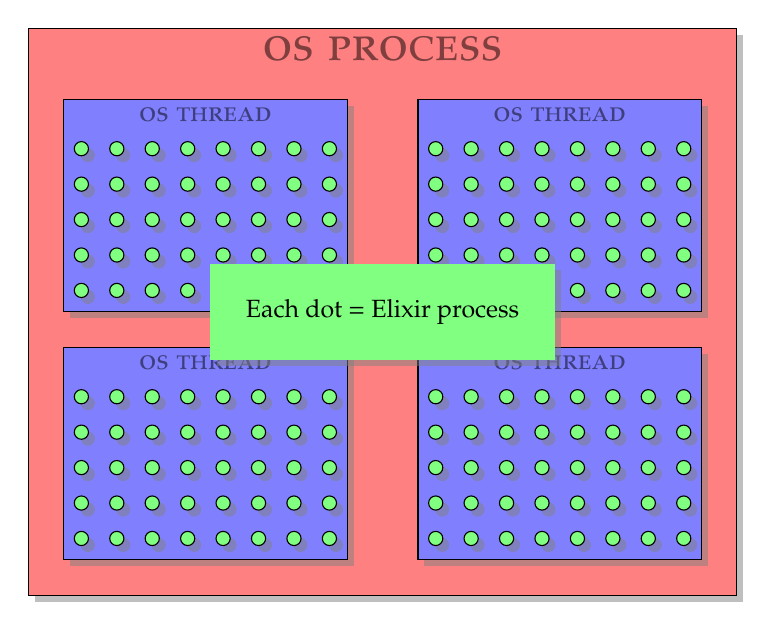
\begin{tikzpicture}[scale=0.9,transform shape,
                            os process/.style={drop shadow,fill=red!50},
                            os process header/.style={opacity=0.5,font=\huge\sc},
                            os thread/.style={drop shadow,fill=blue!50},
                            os thread header/.style={opacity=0.5,font=\large\sc},
                            elixir process/.style={drop shadow,fill=green!50}]
            \draw[os process] (0,0) rectangle (10, 8);
            \node[os process header,anchor=north] at (5,8) {os process};

            \foreach \x/\y in {0.5/0.5,5.5/0.5,0.5/4,5.5/4} {
                \coordinate (p) at (\x,\y);
                \draw[os thread] (p) rectangle ++(4, 3);
                \node[os thread header,anchor=north] at ($ (p) + (2,3) $) {os thread};

                \foreach[evaluate={\i*0.5-0.25} as \dx] \i in {1,...,8} {
                    \foreach[evaluate={\j*0.5-0.2} as \dy] \j in {1,...,5} {
                        \draw[elixir process] (\x+\dx,\y+\dy) circle[radius=0.1cm];
                    }
                }
            }

            \only<2>{
                \node[note] at (5,4) {
                    Each dot = Elixir process
                };
            }
        \end{tikzpicture}
    \end{center}
\end{frame}

\begin{frame}
    \frametitle{Internals}
    \begin{itemize}
        \item BEAM Virtual Machine lives in single OS process
        \item It creates $N$ threads on a machine with $N$ cores
        \item Each threads runs a scheduler
        \item Processes are distributed among these schedulers
        \item Schedulers determine which processes runs
        \item Cooperative "multi-threading" makes it efficient
    \end{itemize}
\end{frame}



\end{document}

%%% Local Variables:
%%% mode: latex
%%% TeX-master: t
%%% End:
